
\begin{frame}{Outline}

We'll be comparing (frequentist) p-values with Bayesian model selection
in a particularly simple setting: testing a point null against a composite
alternative with a scalar parameter.

\begin{itemize}
    \item What is a p-value?
    \item What is Bayesian model selection?
    \item Are they commensurable?  (No)
    \item What now?
\end{itemize}

\end{frame}

%%%%%%%%%%%%%%%%%%%%%%%%%%%%%%%%%%%%%%%%%%%%%%%%%%%%%%%%%%%
%%%%%%%%%%%%%%%%%%%%%%%%%%%%%%%%%%%%%%%%%%%%%%%%%%%%%%%%%%%
%%%%%%%%%%%%%%%%%%%%%%%%%%%%%%%%%%%%%%%%%%%%%%%%%%%%%%%%%%%


\begin{frame}{What is a p-value?}

What is a p-value?

\vspace{1em}

\pause {\Large \textbf{It is garbage. }}

\vspace{1em}

This is the offical position of the American Statistical Association.

\pause
Its executive director writes:

\vspace{1em}

\begin{quote}
``Don’t believe that your p-value gives the probability that chance alone
produced the observed association or effect or the probability that your test
hypothesis is true.  ... Don’t conclude anything about scientific or practical
importance based on statistical significance (or lack thereof).  Don’t. Don’t.
Just...don’t.''  \citep{wasserstein:2019:beyondp}
\end{quote}

\vspace{1em}

\pause Today we will beat this horse a little more.

\end{frame}


%%%%%%%%%%%%%%%%%%%%%%%%%%%%%%%%%%%%%%%%%%%%%%%%%%%%%%%%%%%
%%%%%%%%%%%%%%%%%%%%%%%%%%%%%%%%%%%%%%%%%%%%%%%%%%%%%%%%%%%
%%%%%%%%%%%%%%%%%%%%%%%%%%%%%%%%%%%%%%%%%%%%%%%%%%%%%%%%%%%



\begin{frame}

\begin{figure}[t]
\Large
Whiteboard
\centering
\end{figure}

\end{frame}


\begin{frame}{Table: Fixed Normal prior}

\begin{figure}[t]
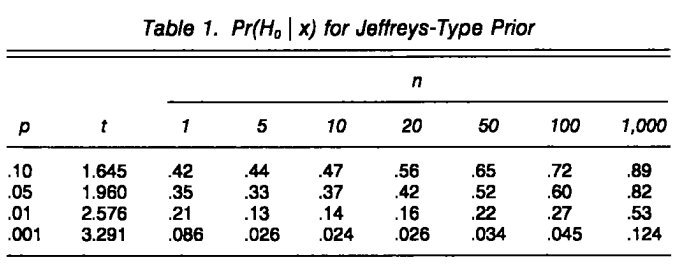
\includegraphics[width=0.8\textwidth]{figures/table1}
\centering
\end{figure}

\end{frame}


% table2 is effectively a duplicate of table5
% \begin{frame}{Tables}
%
% \begin{figure}[t]
% 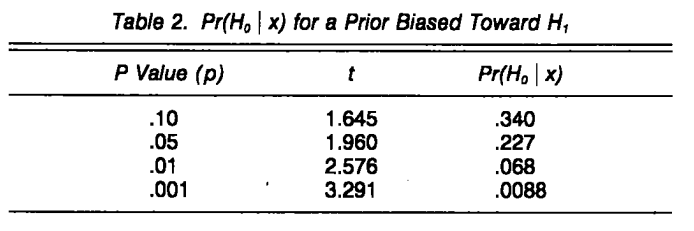
\includegraphics[width=0.8\textwidth]{figures/table2}
% \centering
% \end{figure}
%
% \end{frame}


\begin{frame}{Table: All priors}

\begin{figure}[t]
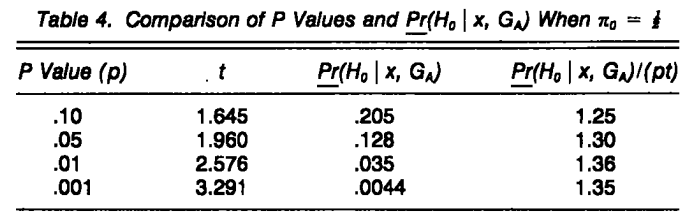
\includegraphics[width=0.8\textwidth]{figures/table4}
\centering
\end{figure}

\end{frame}



\begin{frame}{Table: Symmetric priors centered at $\theta_0$}

\begin{figure}[t]
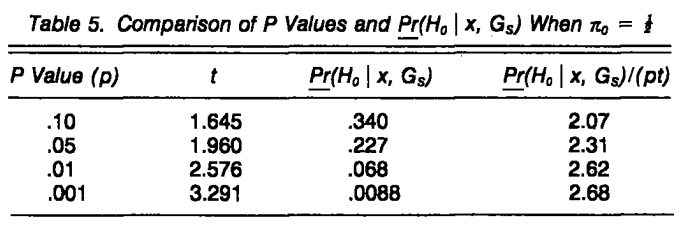
\includegraphics[width=0.8\textwidth]{figures/table5}
\centering
\end{figure}

\end{frame}



\begin{frame}{Table: Unimodal symmetric priors centered at $\theta_0$}

\begin{figure}[t]
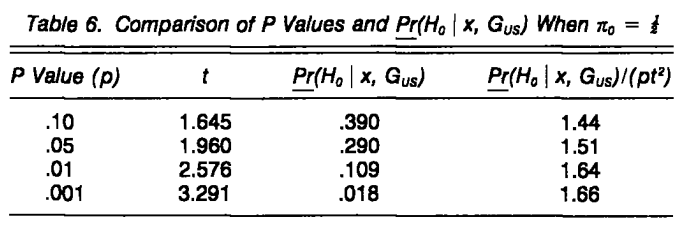
\includegraphics[width=0.8\textwidth]{figures/table6}
\centering
\end{figure}

\end{frame}



\begin{frame}{Table: Normal priors centered at $\theta_0$}

\begin{figure}[t]
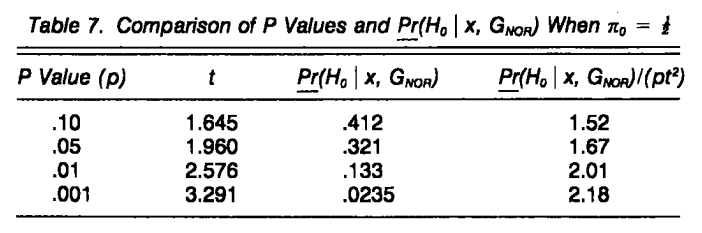
\includegraphics[width=0.8\textwidth]{figures/table7}
\centering
\end{figure}

\end{frame}



\begin{frame}{Figure}

\begin{figure}[t]
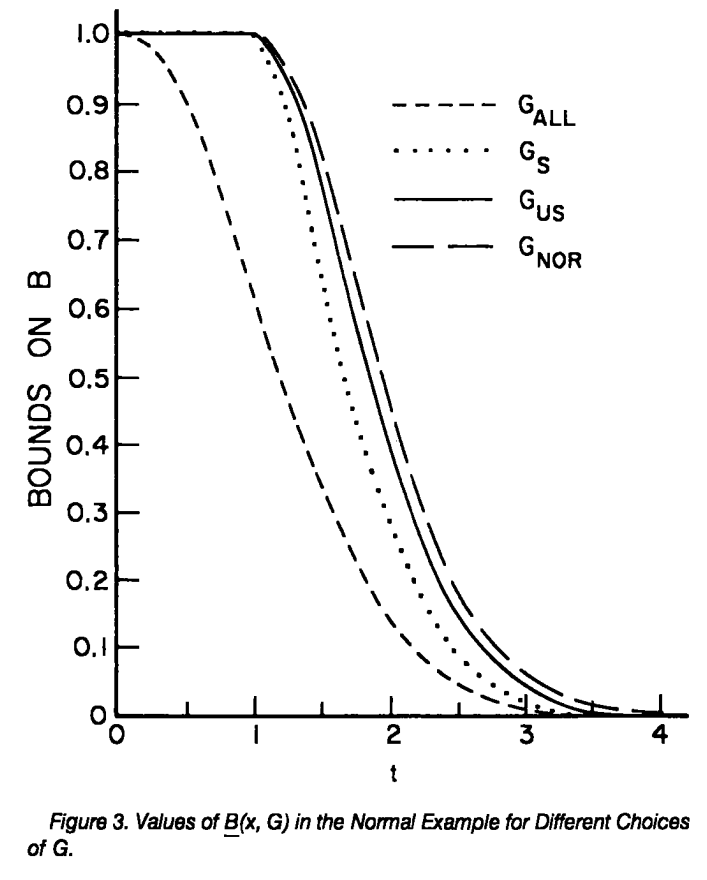
\includegraphics[width=0.65\textheight]{figures/figure3}
\centering
\end{figure}

\end{frame}



\begin{frame}{Figure}

\begin{figure}[t]
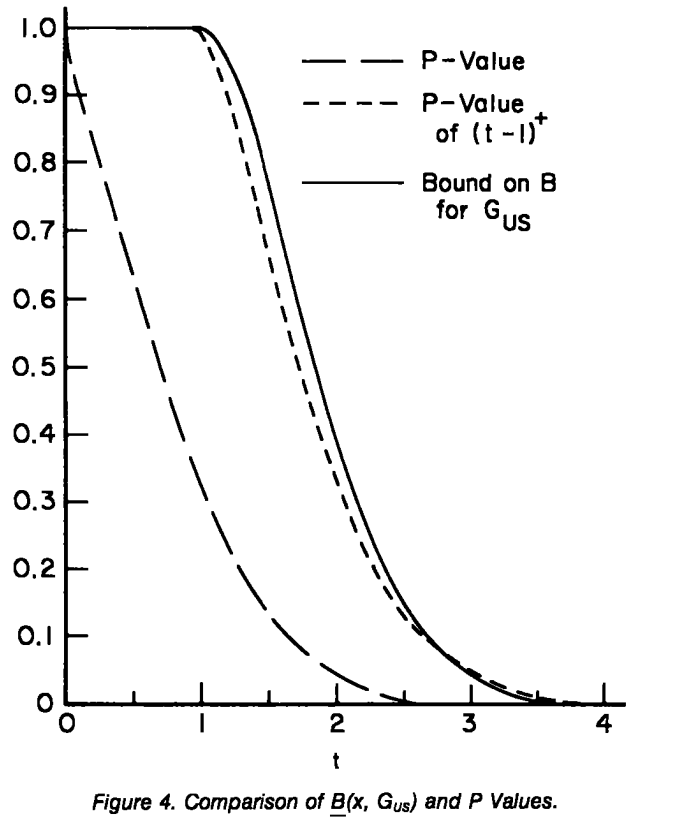
\includegraphics[height=0.8\textheight]{figures/figure4}
\centering
\end{figure}

\end{frame}


\begin{frame}{Table for Cauchy}

\#notalldistributions

\begin{figure}[t]
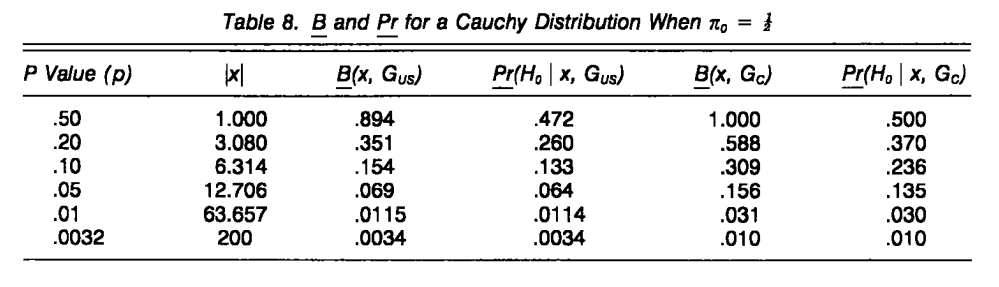
\includegraphics[width=0.8\textwidth]{figures/table8}
\centering
\end{figure}

\end{frame}



\begin{frame}{Where are we at?}

How do p-values and Bayesian model selection stack up in terms of:

\begin{itemize}
    \item Interpretability?
    \item Ease of use?
        \begin{itemize}
        \item Theoretical (understanding behavior)
        \item Analytical (coming up with a design in practice)
        \item Computational (computing what is needed)
        \end{itemize}
    \item Counterintuitive behavior?
        \begin{itemize}
        \item Is counterintuitive behavior possible?
        \item Is counterintuitive behavior detectable?
        \item Is counterintuitive behavior easy to understand?
        \end{itemize}
\end{itemize}
% \begin{figure}[t]
% \begin{tabular}{|c|c|}
%     \hline
%     \textbf{P-values}        &   \textbf{Bayesian model selection} \\ \hline
%     Need to specify fewer things & Need to specify a lot \\
%     (Test statistic and rejection region) & (Full distribution over alternatives) \\ \hline
%
%     Easy to confuse semantically & Means exactly what it says \\
%      & (Full distribution over alternatives) \\ \hline
% \end{tabular}
% \centering
% \end{figure}

\end{frame}
